\documentclass[conference,a4paper]{IEEEtran}
% IEEEtran provides the IEEE layout: two columns, 10 pt Times, section headings
% ("I. INTRODUCTION", "A. Subsection"), "Fig." and "TABLE I" captions, and
% references to subsections printed as "Section III-A".
% Single-column variant: use \documentclass[conference,onecolumn,a4paper]{IEEEtran}
% and set \figwidth below to 0.62\columnwidth.

% ----------------------------------------------------------------- Fonts
\usepackage[T1]{fontenc}
\usepackage[utf8]{inputenc}
% Times text and math. newtx is preferred; mathptmx is a fallback that ships
% with every TeX distribution.
\IfFileExists{newtxtext.sty}
  {\usepackage{newtxtext}\usepackage{newtxmath}}
  {\usepackage{mathptmx}\usepackage{amssymb}}   % amssymb: \mathbb (newtxmath has it built in)
\usepackage{microtype}
% Long file names in \texttt cannot be hyphenated; allow a little extra
% inter-word space instead of letting them stick out into the margin.
\setlength{\emergencystretch}{2em}

% ---------------------------------------------------------------- Content tools
\usepackage{amsmath}
\interdisplaylinepenalty=2500   % recommended by IEEEtran when using amsmath
\usepackage{graphicx}
\usepackage{booktabs}
\usepackage{array}
\usepackage{enumitem}
\usepackage{listings}
\usepackage{xcolor}
\usepackage{balance}   % equal-height columns on the last page (IEEE style)

% Figures generated by assignment_2/plot_results.py. They are designed for a
% 3.5 in column, so \includegraphics[width=\columnwidth] prints them at the
% intended size (see common/plotting_style.md).
\graphicspath{{../results/}}
\newcommand{\figwidth}{\columnwidth}

% Code listings (small, monospaced, light frame). The two listings are floats
% (float=t in each), so a listing is never split across columns or pages.
\lstset{basicstyle=\footnotesize\ttfamily, frame=lines, framesep=3pt,
        columns=fullflexible, keepspaces=true, xleftmargin=0pt, xrightmargin=0pt}

% Links in the deep blue used for the baseline in the figures.
\definecolor{linkblue}{HTML}{1F43B2}
\usepackage[colorlinks=true,linkcolor=linkblue,citecolor=linkblue,urlcolor=linkblue]{hyperref}
% TODO: add your name as pdfauthor.
\hypersetup{pdftitle={Optimised Matrix Multiplication Approaches and Sparse Matrices},
            pdfauthor={}}

% ------------------------------------------------------------- Placeholders
% \TODO{...} prints a red marker in the PDF so no placeholder is forgotten.
\newcommand{\TODO}[1]{\textcolor{red}{\textbf{[TODO: #1]}}}

% ------------------------------------------------------------------ Shortcuts
\newcommand{\bigO}[1]{\mathcal{O}\!\left(#1\right)}
\newcommand{\code}[1]{\texttt{#1}}
\newcommand{\nnz}{\operatorname{nnz}}

% =============================================================================
\title{Optimised Matrix Multiplication Approaches\\and Sparse Matrices}
% TODO: replace the placeholder with your name.
\author{\IEEEauthorblockN{{Javier Ruano Hernández}}
\IEEEauthorblockA{Big Data -- Assignment 2\\
Universidad de Las Palmas de Gran Canaria (ULPGC)\\
% Check that the repository is public (or that the instructor has access).
Code and data: \url{https://github.com/javierruanohdez/big-data-assignments/tree/main/assignment_2}}}

\begin{document}
\maketitle

% =============================================================================
% ABSTRACT
% =============================================================================
\begin{abstract}
We study two ways of reducing the cost of matrix multiplication beyond the
textbook $\bigO{n^3}$ triple loop, in sequential C. Part~A compares two
cache-oriented optimisations, loop reordering (i-k-j) and cache blocking
(tiling), with the i-j-k baseline for $n$ from 100 to 2000. Part~B compares a
Compressed Sparse Row (CSR) multiplication based on Gustavson's algorithm with
the fastest dense kernel at $n = 1000$ for sparsities from 0 to 99.9\%, timing
the dense-to-CSR conversion separately. All kernels read the same inputs,
produce bit-identical results and were validated against a correctly rounded
reference; each configuration ran five times in fresh processes. On the tested
machine, reordering and tiling were 4.5 and 4.4 times faster than the baseline
at $n = 2000$ with no extra memory, and scaled with an exponent of 3.0 against
3.7 for the baseline ($n = 500$--2000). Including the conversion, CSR beat the
tiled kernel from about 44\% sparsity and was 74 and 132 times faster at 99\%
and 99.9\%; above 97\% the conversion cost more than the multiplication itself.
Fill-in followed the model $1-(1-d^2)^n$ within 0.07 percentage points: inputs
with 95\% zeros produced a product with 92\% non-zeros. These results describe
one machine and one configuration.
\end{abstract}

\begin{IEEEkeywords}
matrix multiplication, cache blocking, loop tiling, sparse matrices,
compressed sparse row, fill-in, performance evaluation.
\end{IEEEkeywords}

% =============================================================================
\section{Introduction and Objective}
\label{sec:intro}
% =============================================================================

Assignment~1 showed that the textbook i-j-k matrix multiplication grows faster
than its $n^3$ operation count once the matrices outgrow the caches: time is
increasingly spent waiting for data rather than computing. This report studies
two independent remedies in sequential C. The first keeps all $2n^3$
floating-point operations and only reorders them so that cached data is reused:
loop reordering and cache blocking, or tiling~\cite{lam1991,wolf1991}. The
second stores and multiplies only the non-zeros of sparse
matrices~\cite{gustavson1978}, at the price of indirect indexing, a conversion
from the dense input, and \emph{fill-in}: the product of sparse matrices is
usually much denser than its factors.

\paragraph{Objective} We answer the following research question:

\begin{quote}
\emph{How much can cache-aware loop orders reduce the execution time of dense
matrix multiplication, and from which sparsity does a sparse (CSR)
multiplication outperform the best dense kernel once its overheads are
counted?}
\end{quote}

\begin{enumerate}[label=\textbf{RQ\arabic*.}, leftmargin=3.2em, itemsep=1pt]
  \item \emph{(Part A)} How much faster than the i-j-k baseline are the i-k-j
        and tiled kernels as $n$ grows, and at what memory cost?
  \item \emph{(Part A)} How does their time scale with respect to the $n^3$
        model?
  \item \emph{(Part B)} From which sparsity is CSR, including the conversion,
        faster than the best dense kernel?
  \item \emph{(Part B)} How dense is the product, and does it follow a simple
        probabilistic model?
\end{enumerate}

\paragraph{Contributions and scope} We provide (i)~three dense kernels and one
CSR kernel that perform the same arithmetic on the same inputs with
bit-identical results; (ii)~an input generator with exact, nested sparsity
levels; (iii)~an automated pipeline that validates, runs and analyses Part~A
and Part~B separately; and (iv)~a measurement-based analysis of the
optimisations, the sparse crossover and fill-in. Code and raw data are in the
repository linked on the first page. The results describe one machine
(Section~\ref{sec:environment}). Part~A varies only the loop structure and
Part~B only the storage format, and the two are analysed separately.

% =============================================================================
\section{Background and References}
\label{sec:background}
% =============================================================================

\subsection{Loop Order and the Memory Hierarchy}
For $A, B \in \mathbb{R}^{n \times n}$, the product $C = AB$ is
\begin{equation}
  c_{ij} = \sum_{k=0}^{n-1} a_{ik}\, b_{kj}, \qquad 0 \le i, j < n.
  \label{eq:matmul}
\end{equation}
The direct triple loop takes $\Theta(n^3)$ time, and the three matrices occupy
$24n^2$ bytes. Caches hold data in lines of 64
bytes~\cite{hennessy2017,drepper2007}. In the row-major i-j-k order, the inner
loop reads $B$ down a column with a stride of $8n$ bytes, using one double per
line; once the working set exceeds a cache level, time grows faster than
$n^3$~\cite{lam1991}. Interchanging the two inner loops gives the i-k-j order,
\begin{equation}
  c_{i,:} \;=\; \sum_{k=0}^{n-1} a_{ik}\, b_{k,:},
  \label{eq:ikj}
\end{equation}
whose inner loop reads a row of $B$ and updates a row of $C$ with unit stride,
while $a_{ik}$ stays in a register. Every cache line is fully used and both
streams are easy to prefetch. Each $c_{ij}$ still receives its terms in
increasing $k$, so the result is unchanged. However, all of $B$ is streamed
again for every row $i$: about $n^3$ elements once $B$ exceeds the cache.

\subsection{Cache Blocking (Tiling)}
Tiling applies \eqref{eq:matmul} to $b \times b$ tiles:
\begin{equation}
  C_{IJ} = \sum_{K} A_{IK}\, B_{KJ}.
  \label{eq:tiled}
\end{equation}
A tile product touches $3 \cdot 8b^2$ bytes. If they fit in cache, each element
of a $B$ tile is reused $b$ times, cutting memory traffic from about $n^3$ to
about $2n^3/b$ elements~\cite{lam1991,wolf1991}, i.e.\ 32 times less for
$b = 64$. High-performance BLAS libraries apply this idea at every cache
level~\cite{goto2008}.

\subsection{CSR Format and Gustavson's Algorithm}
Let $d = \nnz/n^2$ be the density of a matrix and $s = 1 - d$ its sparsity.
CSR stores the non-zeros row by row in \code{values}, their columns in
\code{col\_idx}, and the start of each row in \code{row\_ptr}, so row $i$
occupies positions $\code{row\_ptr}[i]$ to
$\code{row\_ptr}[i{+}1]-1$~\cite{saad2003,davis2006}. With 4-byte column
indices it needs $12\,\nnz + 8(n+1)$ bytes, against $8n^2$ for a dense matrix,
so it is smaller when $d < 2/3$. Gustavson's algorithm~\cite{gustavson1978}
evaluates \eqref{eq:ikj} over the non-zeros only,
\begin{equation}
  c_{i,:} \;=\; \sum_{k \,:\, a_{ik} \neq 0} a_{ik}\, b_{k,:},
  \label{eq:gustavson}
\end{equation}
reading $A$ and $B$ by rows, as CSR allows. Row $i$ of $C$ is built in a
\emph{sparse accumulator}~\cite{gilbert1992}: a dense array of $n$ partial sums
plus a list of touched columns. Products are added into it (scatter), then
copied to $C$ and reset (gather). The cost is $\bigO{n + \nnz(A) + F}$, where
\begin{equation}
  F = \sum_{(i,k)\,:\,a_{ik} \neq 0} \nnz(b_{k,:}) \;\approx\; d^2 n^3
  \label{eq:flops}
\end{equation}
is the number of non-zero products for randomly placed non-zeros: a quarter of
the dense work at $s = 0.5$, one hundredth at $s = 0.9$. Each product, however,
needs an index load and a test for new columns, and the size of $C$ is not
known in advance.

\subsection{Fill-in}
\label{sec:bg-fillin}
Barring exact cancellation, $c_{ij} \neq 0$ if some $k$ has $a_{ik} \neq 0$ and
$b_{kj} \neq 0$. For independently placed non-zeros of density $d$, each of the
$n$ products is non-zero with probability $d^2$, so
\begin{equation}
  P(c_{ij} \neq 0) = 1 - (1 - d^2)^n .
  \label{eq:fillin}
\end{equation}
For $n = 1000$ and $d = 0.05$ this gives 0.918. Since \eqref{eq:fillin} is
close to $n d^2$ when $n d^2$ is small, the product is denser than its factors
unless $d \lesssim 1/n$. Fill-in is a central concern of sparse direct
methods~\cite{davis2006}.

% =============================================================================
\section{Methodology}
\label{sec:method}
% =============================================================================

\subsection{Experimental Environment}
\label{sec:environment}
All measurements were taken on the machine described in
Table~\ref{tab:environment}, with other applications closed and the computer
connected to mains power.

\begin{table}[t]
  \centering
  \caption{Hardware and software environment}
  \label{tab:environment}
  \footnotesize
  % Sources: lscpu, free, /etc/os-release, uname, gcc --version, python3 --version,
  % pip show. lscpu reports cache totals over the 4 cores; the per-core sizes are
  % the ones a single-threaded kernel uses. Clock: CPU specification (lscpu under
  % WSL does not report it); same CPU as in Assignment 1.
  \begin{tabular}{@{}l>{\raggedright\arraybackslash}p{0.64\columnwidth}@{}}
    \toprule
    \textbf{Item} & \textbf{Value} \\
    \midrule
    CPU model               & AMD Ryzen AI 5 330 w/ Radeon 820M \\
    Cores / logical threads & 4 cores / 8 threads \\
    Clock                   & 2.0~GHz base; boost up to 4.5~GHz (1 Zen~5 core)
                              and 3.4~GHz (3 Zen~5c cores) \\
    Caches                  & L1d 192~KiB, L1i 128~KiB, L2 4~MiB (i.e.\ 48~KiB,
                              32~KiB and 1~MiB per core); L3 8~MiB shared \\
    RAM                     & 15~GiB (available to WSL~2) \\
    Operating system        & Ubuntu 26.04 LTS on WSL2 (Windows Subsystem for Linux) \\
    Kernel                  & 6.18.33.2-microsoft-standard-WSL2 \\
    C compiler              & GCC 15.2.0 \\
    Python                  & CPython 3.14.4 \\
    Analysis                & pandas 3.0.3, Matplotlib 3.10.9 \\
    \bottomrule
  \end{tabular}
\end{table}

\subsection{Implementations}
\label{sec:impl}
All kernels are sequential C with 64-bit doubles, flat row-major arrays, and
the input loader and timer of Assignment~1. \code{dense\_mult.c} contains the
\textbf{baseline} (the Assignment~1 i-j-k kernel, unchanged), the
\textbf{reordered} i-k-j kernel, and the \textbf{tiled} kernel with $b = 64$,
whose tile loops run in the order $ii$-$jj$-$kk$ with i-k-j inside, so that each
tile of $C$ is completed while it stays in cache (Listing~\ref{lst:dense}).
The last two accumulate into $C$ and clear it first ($n^2$ stores, less than
0.1\% of the work for $n \ge 1000$). All three add the terms of each $c_{ij}$
in increasing $k$ and produce bit-identical results. Two details mattered.
First, the kernels are compiled as separate functions (\code{noinline}): when
GCC inlined the six-loop tiled kernel into \code{main()}, it reloaded a pointer
from the stack in every inner iteration, which made it about 2.5 times slower
in a development test. Second, the result is filled with NaN before the timer
starts, which maps its memory pages in advance and exposes any element a kernel
fails to write.

\begin{lstlisting}[language=C, float=t, caption={Reordered and tiled kernels (simplified). Both start from $C = 0$.}, label=lst:dense, captionpos=b]
/* reordered: i-k-j */
for (i = 0; i < n; i++)
 for (k = 0; k < n; k++)
  for (j = 0; j < n; j++)
   c[i*n + j] += a[i*n + k] * b[k*n + j];
/* tiled: tiles ii-jj-kk, i-k-j inside each */
for (ii = 0; ii < n; ii += bs)
 for (jj = 0; jj < n; jj += bs)
  for (kk = 0; kk < n; kk += bs)
   for (i = ii; i < min(ii+bs, n); i++)
    for (k = kk; k < min(kk+bs, n); k++)
     for (j = jj; j < min(jj+bs, n); j++)
      c[i*n + j] += a[i*n + k] * b[k*n + j];
\end{lstlisting}

\code{sparse\_mult.c} reads the same dense file, converts $A$ and $B$ to CSR
(32-bit column indices, 64-bit row pointers) and multiplies them
(Listing~\ref{lst:csr}). The \emph{conversion} makes two passes per matrix: it
counts the non-zeros of each row into \code{row\_ptr}, allocates the other
arrays exactly, and copies the non-zeros with sorted columns. The
\emph{multiplication} is Gustavson's algorithm with a sparse accumulator.
Because the size of $C$ is unknown, it is bounded in $\bigO{\nnz(A)}$ time by
$\sum_i \min\bigl(n, \sum_{k:\,a_{ik}\neq 0} \nnz(b_{k,:})\bigr)$, which was
within 10\% of $\nnz(C)$ for our inputs, and $C$ is allocated once. Exact
cancellations are dropped, so the reported $\nnz(C)$ is exact; the columns
within a row of $C$ stay in first-touch order. Since the columns of $A$ are
sorted, \code{acc[j]} receives its terms in increasing $k$, and $C$ is
identical to the dense result. Both programs validate the input header and
release all memory on every error path.

\begin{lstlisting}[language=C, float=t, caption={Gustavson's algorithm with a sparse accumulator (simplified). \code{acc} starts at 0, \code{mark} at $-1$.}, label=lst:csr, captionpos=b]
for (i = 0; i < n; i++) {
  t = 0;                                /* scatter */
  for (p = A.ptr[i]; p < A.ptr[i+1]; p++) {
    k = A.col[p];
    for (q = B.ptr[k]; q < B.ptr[k+1]; q++) {
      j = B.col[q];
      if (mark[j] != i) { mark[j] = i; list[t++] = j; }
      acc[j] += A.val[p] * B.val[q];
    }
  }
  for (u = 0; u < t; u++) {             /* gather */
    j = list[u];
    if (acc[j] != 0.0) {
      C.col[nz] = j;  C.val[nz++] = acc[j];
    }
    acc[j] = 0.0;
  }
  C.ptr[i+1] = nz;
}
\end{lstlisting}

\subsection{Inputs and Experimental Design}
\label{sec:design}
Inputs use the binary format and generator of Assignment~1
(\code{common/\allowbreak data\_\allowbreak generator.py}): $n$, followed by $A$
and $B$ as little-endian doubles drawn uniformly from $[-1, 1)$, with a seed
derived from 42 and $n$. For a target sparsity $s$, the generator zeroes exactly
$\operatorname{round}(s\, n^2)$ entries per matrix at positions drawn by a
separate seeded generator (a partial Fisher--Yates shuffle). The sparsity axis
is therefore exact, the non-zeros keep their dense values, the levels are
nested (the zeros at $s = 0.9$ are a subset of those at $s = 0.95$), and $s = 0$
reproduces the Assignment~1 inputs bit for bit. Sparse inputs keep the dense
format, so both programs read identical files and the cost of the conversion is
explicit.

Two experiments are run and analysed separately (Table~\ref{tab:parameters}).
\textbf{Part~A} runs the three dense kernels on dense inputs up to $n = 2000$,
where one matrix occupies 30.5~MB, far beyond the 8~MB L3 cache. \textbf{Part~B}
runs the tiled and CSR kernels at $n = 1000$ for twelve sparsities, including
the levels suggested by the guidelines (50, 90, 95 and 99\%) and a finer grid
near the expected crossover. CSR is compared with the tiled kernel, the fastest
dense kernel at $n = 1000$ in Part~A; comparing it with the baseline would
credit the loop-order effect of Part~A to sparse storage
(Section~\ref{sec:disc-b}). All kernels are compiled with \code{gcc -O2}, as in
Assignment~1. \code{-O3} would auto-vectorize the unit-stride loops of the
optimised kernels, but not the baseline's sequential sum (which needs
\code{-ffast-math}), and would mix a compiler effect into the comparison.

\begin{table}[t]
  \centering
  \caption{Fixed experimental parameters}
  \label{tab:parameters}
  \footnotesize
  \begin{tabular}{@{}l>{\raggedright\arraybackslash}p{0.70\columnwidth}@{}}
    \toprule
    \textbf{Parameter} & \textbf{Value} \\
    \midrule
    Part A      & $n$ = 100, 250, 500, 1000, 2000; $s = 0$; baseline (i-j-k),
                  reordered (i-k-j), tiled ($b = 64$) \\
    Part B      & $n = 1000$; $s$ = 0, 0.3, 0.4, 0.45, 0.5, 0.6, 0.7, 0.8, 0.9,
                  0.95, 0.99, 0.999; tiled vs.\ CSR (Gustavson) \\
    Repetitions & 5 per configuration, each in a fresh process; 300 s budget per run \\
    Inputs      & uniform in $[-1,1)$, exact zeros, base seed 42, shared binary files \\
    Compiler    & \code{gcc -O2 -std=c11 -Wall -Wextra} (all kernels) \\
    Timer       & \code{clock\_gettime(CLOCK\_MONOTONIC)} \\
    Memory      & peak RSS (GNU \code{time -v}); size of the CSR arrays \\
    \bottomrule
  \end{tabular}
\end{table}

\subsection{Measurement Protocol}
The dense program times only the kernel call; input loading, allocating and
pre-faulting the result, and process start-up are excluded. The CSR program
has \textbf{two separate timed regions}: the conversion of $A$ and $B$,
including the allocation of the CSR arrays (\code{conversion\_time\_s}), and
the multiplication, including the size bound and the allocation of $C$ and of
the accumulator (\code{time\_s}), because a sparse kernel cannot know its output
size in advance. All times come from \code{CLOCK\_MONOTONIC} and were recorded
with 1~$\mu$s resolution in this data set.
% The programs now print nanoseconds (commit 8d8bc14); the measurements in
% results/measurements.csv were taken with the previous build (6 decimals).
% If you re-run the benchmark, change "1 us" accordingly.
A harness (\code{run\_benchmark.py}) runs every repetition in a fresh process
and records the peak resident set size (RSS) with GNU \code{time -v}. For CSR,
the RSS includes the dense input buffers ($16n^2$ bytes, 15.3~MB at
$n = 1000$), so the size of the CSR arrays of $A$, $B$ and $C$ is reported as
well. Runs exceeding the 300-s budget are recorded as timeouts. Since all
kernels produce bit-identical results, a run whose checksum differs from the
first one recorded for its input file would be flagged as a mismatch and
excluded.

\subsection{Validation and Statistical Analysis}
Before benchmarking, \code{verify\_correctness.py} runs the four kernels on
eight cases: $A \times I$, $A \times 0$, a hand-computed $3 \times 3$ product,
random $n = 10$, and random $n = 100$ at $s \in \{0, 0.5, 0.9, 0.99\}$, which
exercise full and partial tiles and, at $s = 0.99$, many empty rows. Since
IEEE~754 addition is not associative~\cite{ieee754}, each result is compared
with a correctly rounded \code{math.fsum} reference using the tolerances of
Assignment~1, derived from the dot-product error bound~\cite{higham2002}: an
element passes if
\begin{equation}
  |x - x_{\text{ref}}| \le \tau_{\text{abs}} + \tau_{\text{rel}}\, |x_{\text{ref}}|,
\end{equation}
with $\tau_{\text{rel}} = 10^{-12}$, $\tau_{\text{abs}} = 100\, n^2 u$ and
$u = 2^{-53}$. For CSR, the reported non-zero counts must also be exact. All 32
checks passed: the identity, zero and $3 \times 3$ cases were reproduced
exactly, the largest error was $1.1 \times 10^{-14}$ (random case, $n = 100$),
four orders of magnitude below $\tau_{\text{abs}}$, and every result was
bit-identical to the baseline's.

We report medians and interquartile ranges (IQR $= Q_3 - Q_1$) over the five
repetitions~\cite{georges2007,kalibera2013}. Speed-ups are ratios of medians,
and the scaling exponent $b$ is the slope of $\log t$ versus $\log n$ (model:
3). The CSR total time adds conversion and multiplication per run. The
crossover $s^*$ starts from the lowest measured level $s_i$ from which CSR beats
tiled at every higher level, and interpolates
$r = \ln(t_{\text{CSR}} / t_{\text{tiled}})$ linearly between $s_{i-1}$ and
$s_i$:
\begin{equation}
  s^* = s_{i-1} + (s_i - s_{i-1})\, \frac{r_{i-1}}{r_{i-1} - r_i}.
  \label{eq:crossover}
\end{equation}
The same rule locates the sparsity from which the conversion costs more than
the multiplication. All statistics and figures are produced by
\code{plot\_results.py} from the raw data.

% =============================================================================
\section{Results}
\label{sec:results}
% =============================================================================

% All numbers in Sections IV-VI are computed from results/measurements.csv
% (195 runs, data of commit b23466e). Recompute them if you re-run the benchmark.
All 195 runs (75 in Part~A, 120 in Part~B) completed within the time budget,
with no timeouts, errors or checksum mismatches. Throughout, 1~MB $= 2^{20}$
bytes.

\subsection{Part A: Dense Optimisations}
\label{sec:res-a}

\begin{figure}[t]
  \centering
  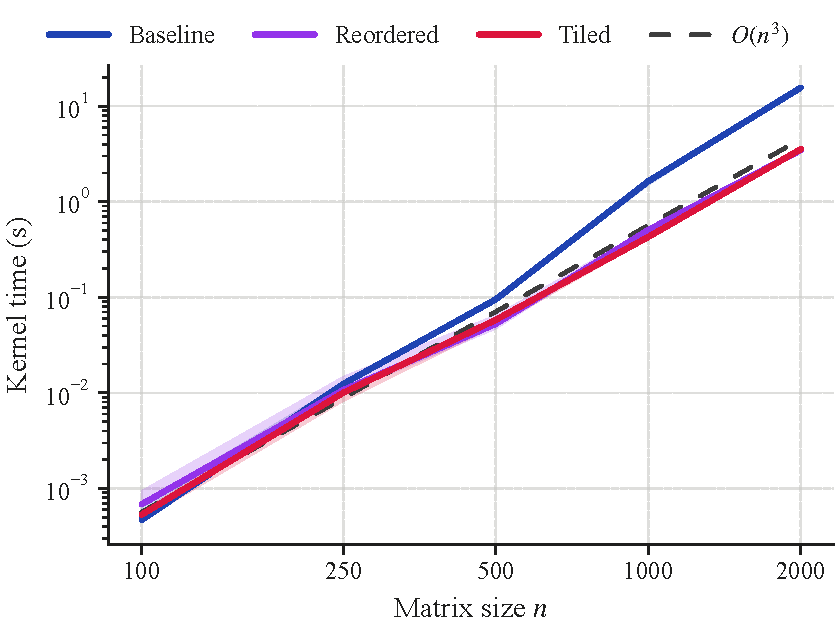
\includegraphics[width=\figwidth]{part_a_time_vs_size.pdf}
  \caption{Part A: median kernel time over five runs vs.\ $n$ (log-log), with
           interquartile-range bands. Dashed: slope~3 ($\propto n^3$).}
  \label{fig:a-time}
\end{figure}

\begin{figure}[t]
  \centering
  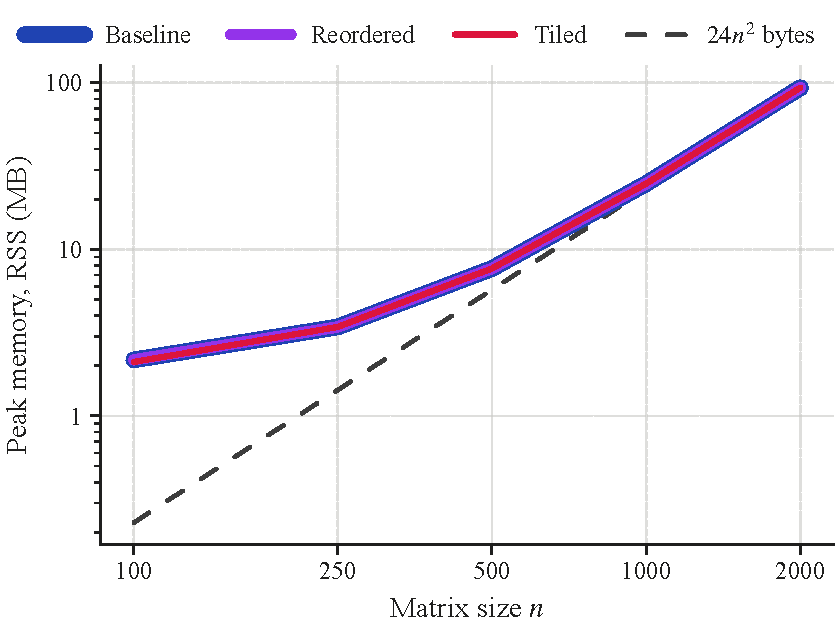
\includegraphics[width=\figwidth]{part_a_memory_vs_size.pdf}
  \caption{Part A: median peak RSS vs.\ $n$ (log-log). The three curves
           coincide (drawn with decreasing widths to keep all visible).
           Dashed: size of the three matrices, $24n^2$ bytes.}
  \label{fig:a-memory}
\end{figure}

\begin{table}[t]
  \centering
  \caption{Part A: median and IQR of the kernel time over five runs,
           speed-up over the baseline and median peak RSS}
  \label{tab:a-summary}
  \footnotesize
  \setlength{\tabcolsep}{4.5pt}
  % Values computed from results/measurements.csv (same statistics as results_summary.md).
  \begin{tabular}{@{}rlrrrr@{}}
    \toprule
    & & \multicolumn{2}{c}{\textbf{Time (s)}} & & \textbf{RSS} \\
    \cmidrule(lr){3-4}
    $n$ & Kernel & Median & IQR & Speed-up & (MB) \\
    \midrule
    100  & Baseline  & 0.000468 & 0.00026 & 1.00 & 2.17 \\
         & Reordered & 0.000683 & 0.00031 & 0.69 & 2.17 \\
         & Tiled     & 0.000531 & 0.00013 & 0.88 & 2.11 \\
    \midrule
    250  & Baseline  & 0.01241 & 0.0010 & 1.00 & 3.42 \\
         & Reordered & 0.01071 & 0.0051 & 1.16 & 3.42 \\
         & Tiled     & 0.01004 & 0.0030 & 1.24 & 3.42 \\
    \midrule
    500  & Baseline  & 0.09505 & 0.00055 & 1.00 & 7.67 \\
         & Reordered & 0.05268 & 0.019 & 1.80 & 7.67 \\
         & Tiled     & 0.05811 & 0.0098 & 1.64 & 7.67 \\
    \midrule
    1000 & Baseline  & 1.638 & 0.16 & 1.00 & 24.80 \\
         & Reordered & 0.5058 & 0.036 & 3.24 & 24.80 \\
         & Tiled     & 0.4279 & 0.029 & 3.83 & 24.80 \\
    \midrule
    2000 & Baseline  & 15.61 & 0.094 & 1.00 & 93.42 \\
         & Reordered & 3.468 & 0.13 & 4.50 & 93.42 \\
         & Tiled     & 3.548 & 0.13 & 4.40 & 93.55 \\
    \bottomrule
  \end{tabular}
\end{table}

\paragraph{Execution time} For $n \le 250$, the three kernels are within a
factor of 1.5 of each other and their order changes with $n$; at $n = 100$
the baseline is even the fastest (0.47~ms, against 0.68~ms for reordered and
0.53~ms for tiled; Fig.~\ref{fig:a-time}, Table~\ref{tab:a-summary}). From $n = 500$ the
optimised kernels lead by a growing margin: reordering is 1.80, 3.24 and 4.50
times faster than the baseline at $n = 500$, 1000 and 2000, and tiling 1.64,
3.83 and 4.40 times. At $n = 2000$ the baseline takes 15.6~s and both optimised
kernels about 3.5~s. The fitted exponents are 3.48, 2.84 and 2.90 (baseline,
reordered, tiled) over all sizes, and 3.68, 3.02 and 2.97 for $n = 500$--2000:
the optimised kernels follow the cubic model, the baseline does not. Per
multiply-add ($t/n^3$), the baseline costs 0.76, 1.64 and 1.95~ns at
$n = 500$, 1000 and 2000, the optimised kernels 0.42--0.51~ns. As in
Assignment~1, the largest jump of the baseline is between $n = 500$ and 1000
(a factor of 17.2 instead of~8). Tiling is 10\% slower than reordering at
$n = 500$, 15\% faster at $n = 1000$ (0.428 vs.\ 0.506~s) and 2\% slower at
$n = 2000$ (3.55 vs.\ 3.47~s). For $n \ge 1000$ the IQR is at most 10\% of the
median (3.8\% at $n = 2000$); for shorter kernels it reaches 55\%. The largest
size finished well within the budget (slowest run: 16.0~s), so the largest
feasible $n$ is at least 2000.

\paragraph{Memory} The three kernels have the same peak RSS within 0.13~MB at
every size (Fig.~\ref{fig:a-memory}): 24.80~MB at $n = 1000$ and 93.4~MB at
$n = 2000$, only 2\% above the 91.6~MB of the three matrices. Neither
optimisation uses additional memory.

\subsection{Part B: Sparse Storage}
\label{sec:res-b}

\begin{figure}[t]
  \centering
  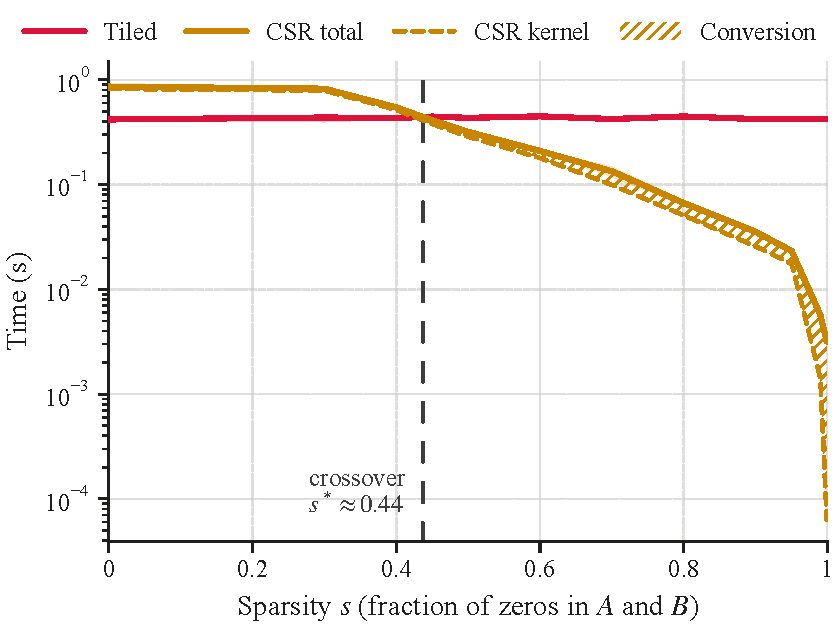
\includegraphics[width=\figwidth]{part_b_time_vs_sparsity.pdf}
  \caption{Part B ($n = 1000$): median time vs.\ sparsity $s$ (log scale).
           CSR total = conversion + multiplication, with IQR band; dashed: CSR
           multiplication alone; hatched: conversion, stacked on top of it.
           Vertical line: crossover $s^* \approx 0.44$.}
  \label{fig:b-time}
\end{figure}

\begin{figure}[t]
  \centering
  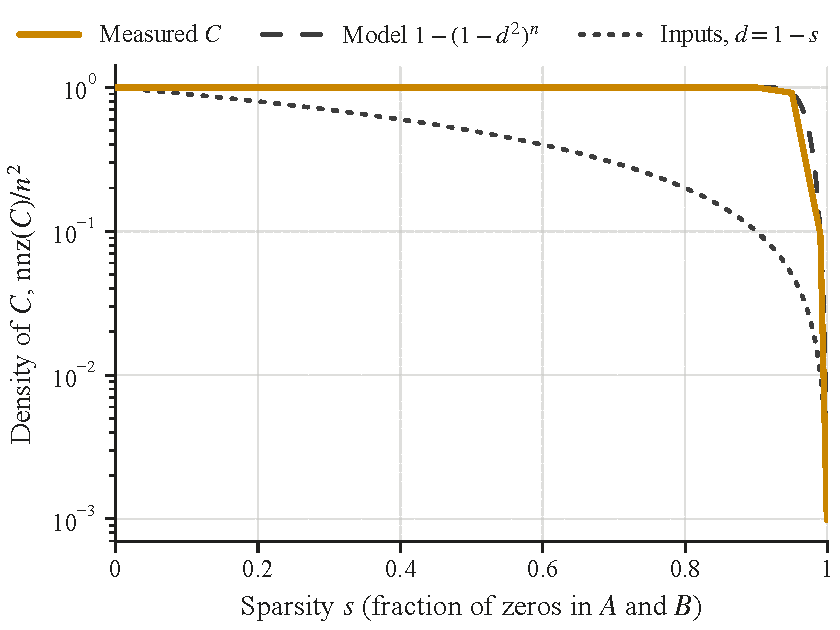
\includegraphics[width=\figwidth]{part_b_fill_in.pdf}
  \caption{Part B ($n = 1000$): density of the product, $\nnz(C)/n^2$, vs.\ $s$
           (log scale), with model~\eqref{eq:fillin} (dashed) and the input
           density $d = 1 - s$ (dotted). Between 0.95 and 0.99 the straight
           line joining the measured levels lies below the curved model only
           because of the interpolation.}
  \label{fig:b-fill}
\end{figure}

\begin{table}[t]
  \centering
  \caption{Part B ($n = 1000$): median times over five runs and speed-up of
           CSR (total) over tiled}
  \label{tab:b-time}
  \footnotesize
  \setlength{\tabcolsep}{3.6pt}
  % Values computed from results/measurements.csv (same statistics as results_summary.md).
  % "Total" is the median of per-run sums, so it can differ slightly from the
  % sum of the two medians to its left.
  \begin{tabular}{@{}lrrrrr@{}}
    \toprule
    & \textbf{Tiled} & \multicolumn{3}{c}{\textbf{CSR (s)}} & \\
    \cmidrule(lr){3-5}
    $s$ & (s) & Multiply & Conversion & Total & Speed-up \\
    \midrule
    0     & 0.4192 & 0.8196   & 0.02999  & 0.8634   & 0.49 \\
    0.3   & 0.4374 & 0.7904   & 0.03093  & 0.8247   & 0.53 \\
    0.4   & 0.4331 & 0.5176   & 0.02976  & 0.5463   & 0.79 \\
    0.45  & 0.4467 & 0.3789   & 0.03259  & 0.4122   & 1.08 \\
    0.5   & 0.4343 & 0.2870   & 0.03498  & 0.3193   & 1.36 \\
    0.6   & 0.4489 & 0.1798   & 0.03003  & 0.2098   & 2.14 \\
    0.7   & 0.4233 & 0.09936  & 0.03071  & 0.1343   & 3.15 \\
    0.8   & 0.4477 & 0.05085  & 0.01579  & 0.06664  & 6.72 \\
    0.9   & 0.4231 & 0.02576  & 0.009702 & 0.03546  & 11.9 \\
    0.95  & 0.4268 & 0.01756  & 0.005746 & 0.02331  & 18.3 \\
    0.99  & 0.4244 & 0.001435 & 0.004100 & 0.005714 & 74.3 \\
    0.999 & 0.4203 & 0.000063 & 0.003117 & 0.003180 & 132 \\
    \bottomrule
  \end{tabular}
\end{table}

\begin{table}[t]
  \centering
  \caption{Part B ($n = 1000$): non-zeros and density of the product, CSR
           storage of $A$, $B$ and $C$, and peak RSS of the CSR program
           (selected levels; dense storage of the three matrices: 22.89~MB)}
  \label{tab:b-fill}
  \footnotesize
  \setlength{\tabcolsep}{3.6pt}
  % Model: 1 - (1 - d^2)^n with d = 1 - s. All levels are in results_summary.md.
  \begin{tabular}{@{}lrrrrr@{}}
    \toprule
    & & \multicolumn{2}{c}{\textbf{Density of $C$}} & \textbf{CSR} & \textbf{RSS} \\
    \cmidrule(lr){3-4}
    $s$ & $\nnz(C)$ & Measured & Model & (MB) & (MB) \\
    \midrule
    0     & 1\,000\,000 & 1.00000 & 1.00000 & 34.36 & 39.80 \\
    0.5   & 1\,000\,000 & 1.00000 & 1.00000 & 22.91 & 28.30 \\
    0.7   & 1\,000\,000 & 1.00000 & 1.00000 & 18.33 & 23.68 \\
    0.9   & 999\,948    & 0.99995 & 0.99996 & 13.76 & 19.05 \\
    0.95  & 917\,481    & 0.91748 & 0.91817 & 11.67 & 17.93 \\
    0.99  & 94\,911     & 0.09491 & 0.09517 & 1.34  & 17.05 \\
    0.999 & 981         & 0.00098 & 0.00100 & 0.06  & 16.80 \\
    \bottomrule
  \end{tabular}
\end{table}

\paragraph{Execution time} The tiled kernel takes 0.419--0.449~s at every
sparsity, since it multiplies zeros like any other value
(Fig.~\ref{fig:b-time}, Table~\ref{tab:b-time}). The CSR total falls from
0.863~s at $s = 0$, where CSR is 2.06 times slower than tiled, to 3.18~ms at
$s = 0.999$, but by less than 5\% between $s = 0$ and $0.3$, although $F$
halves. CSR overtakes tiled between $s = 0.4$ (0.546 vs.\ 0.433~s) and
$s = 0.45$ (0.412 vs.\ 0.447~s); \eqref{eq:crossover} gives $s^* = 0.437$, or
0.426 without the conversion. Beyond it, CSR is 1.36, 11.9, 18.3, 74 and 132
times faster at $s = 0.5$, 0.9, 0.95, 0.99 and 0.999. The conversion takes
30--35~ms up to $s = 0.7$ and 3.1~ms at $s = 0.999$. Its share of the CSR total
grows from 3.5\% at $s = 0$ to 11\% at 0.5, 27\% at 0.9, 72\% at 0.99 and 98\%
at 0.999, and it exceeds the multiplication from $s \approx 0.971$.

\paragraph{Fill-in and memory} The product has at least 99.995\% non-zeros up
to $s = 0.9$ (Fig.~\ref{fig:b-fill}, Table~\ref{tab:b-fill}). At $s = 0.95$,
inputs with 5\% non-zeros produce 91.75\% non-zeros, 18.3 times the input
density; at $s = 0.99$, 9.49\%; at $s = 0.999$, 981 non-zeros, slightly fewer
than each input (1000). Model~\eqref{eq:fillin} predicts 91.82\%, 9.52\% and
999.5, i.e.\ agreement within 0.07 percentage points. The CSR storage of $A$,
$B$ and $C$ is 34.4~MB at $s = 0$, 1.5 times the 22.9~MB of dense storage,
equals it at $s = 0.5$, and falls to 13.8~MB at $s = 0.9$ and 1.3~MB at
$s = 0.99$. The RSS of the CSR program falls from 39.8 to 16.8~MB and is below
that of the tiled program (24.8~MB) only from $s = 0.7$.

% =============================================================================
\section{Discussion}
\label{sec:discussion}
% =============================================================================

\subsection{Part A: Cache Effects}
\label{sec:disc-a}
The dense kernels perform identical operations, so their differences come from
memory access. The baseline's cost per multiply-add doubles between $n = 500$
and 1000, when its working set leaves the caches
(Table~\ref{tab:environment}). A column of $B$ spans $64n$ bytes of cache
lines: 31~KB at $n = 500$, inside the 48~KB L1 data cache of a core, but 62~KB
at $n = 1000$. More importantly, $B$, which is read in full for every row of
$C$, grows from 1.9 to 7.6~MB, practically the whole 8~MB L3, which it shares
with $A$ and $C$. At $n = 2000$, $B$ (30.5~MB) is almost four times the L3 and
must come from main memory, and each inner step waits for a cache line that
delivers one useful double out of eight. The reordered and tiled kernels keep
0.42--0.51~ns per multiply-add for $n \ge 500$: their unit-stride loops use
every byte of each line and the prefetcher streams $B$ and $C$ ahead of use, so
their exponent stays at 3.0 and their speed-up grows with $n$. For
$n \le 250$, $B$ (78 and 488~KB) fits in the 1~MB L2 of a core, the baseline
pays no penalty, and the extra work of the optimised kernels (clearing $C$,
loading and storing it in every iteration, tile loops) leaves them no faster,
within the large noise of sub-millisecond kernels.

Tiling did not beat reordering at \code{-O2}, although it moves far less data.
At $n = 2000$, reordering streams $B$ once per row of $C$, about 64~GB in
3.47~s (18.5~GB/s), whereas $64 \times 64$ tiles would need about 2~GB. If
memory bandwidth were the limit, tiling would win; instead, both run at about
0.43~ns, or 1.5--2 cycles per multiply-add at 3.4--4.5~GHz. Our interpretation
is that the scalar inner loop (two loads, a store, a multiplication, an
addition and loop control, not vectorized at \code{-O2}) limits both kernels:
tiling saves a cost that is not the bottleneck and adds loop overhead (its
inner loops have only 64 iterations). It should pay off once SIMD makes the
loop faster; a preliminary single-run \code{-O3} check outside the protocol
pointed this way (tiled 1.6--1.7~s against 1.9--2.4~s for reordered at
$n = 2000$).
% Source: development notes; single runs in a Linux VM on the same laptop with
% a different GCC version. Not part of measurements.csv - remove if unwanted.
The 10--15\% differences at $n = 500$ and 1000 are within the variability of
this CPU (Section~\ref{sec:limits}). Both optimisations are free in memory, but
not immune to code generation: the 2.5-fold inlining slowdown
(Section~\ref{sec:impl}) could have erased their benefit.

\subsection{Part B: The Sparse Advantage and Its Price}
\label{sec:disc-b}
\paragraph{Choice of comparator} At $s = 0$, CSR performs all $10^9$ products
plus indexing, yet its multiplication (0.82~s) is 2.0 times faster than the
Part~A baseline on the same input file (1.64~s). Gustavson's
algorithm~\eqref{eq:gustavson} is the i-k-j order restricted to non-zeros: it
reads rows of $B$ sequentially and sweeps the accumulator from left to right,
inheriting the loop-order benefit of Part~A. Against the reordered kernel
(0.51~s) it is 1.6 times slower, the pure cost of sparse indexing. Against the
baseline, CSR would win at every sparsity; only the fastest dense kernel
isolates the benefit of skipping zeros.

\paragraph{Crossover} CSR performs $F \approx d^2 n^3$ products; at
$s^* = 0.437$, $d^2 = 0.32$, so a sparse product may cost about three dense
multiply-adds. Indeed, the tiled kernel spends 0.43~ns per multiply-add and CSR
1.44 and 1.25~ns per product at $s = 0.4$ and 0.45. This cost is lowest at
$s = 0$ (0.82~ns), where the rows of $B$ are complete and the accumulator is
swept strictly in order, and rises to 1.4--1.6~ns at $s = 0.3$--0.4, where the
entries of each row are irregularly spaced; hence CSR hardly speeds up until
$s = 0.3$. At a constant 0.82~ns per product, the crossover would lie near
$s = 0.28$. The crossover is therefore machine-specific: on a cloud virtual
machine during development, the same pipeline placed it at about 0.26.

\paragraph{Conversion} The $\bigO{n^2}$ conversion is only 5--8\% of the CSR
time near the crossover and shifts it by one percentage point. As the
multiplication shrinks with $d^2$, however, the conversion dominates beyond
$s \approx 0.97$ (98\% at 0.999), limiting the speed-up there to 132 instead
of about 6700 for the multiplication alone. It is amortized when matrices are
created sparse or reused, which our dense-input protocol does not allow. Its
peak around $s = 0.5$ (35 vs.\ 30~ms at $s = 0$) is consistent with, but does
not prove, mispredicted branches in the test for zero.

\paragraph{Fill-in} The product is far denser than its factors, as
\eqref{eq:fillin} predicts: practically dense up to $s = 0.9$ and 18 times
denser than the inputs at $s = 0.95$. In CSR, each non-zero of $C$ takes 12
bytes instead of 8 (11.4 vs.\ 7.6~MB for a full $C$), so the CSR storage
exceeds the dense storage up to $s \approx 0.5$, is still 60\% of it at
$s = 0.9$, and saves memory substantially only for $s \ge 0.99$ (1.3 vs.\
22.9~MB). The gather step also writes every non-zero of $C$, so the real cost
is $\bigO{n + \nnz(A) + F + \nnz(C)}$. At $s = 0.99$, $\nnz(C)$ (about
95\,000) is comparable to $F$ (about 100\,000), and with per-row overheads the
cost per product rises to 2.6~ns at $s = 0.9$ and 14~ns at $s = 0.99$. Since
\eqref{eq:fillin} is close to $n d^2$ for small $d$, random sparse products
stay sparser than their inputs only for $d < 1/n$, i.e.\ above 99.9\% sparsity
at $n = 1000$, so repeated products such as matrix powers quickly become dense.
Finally, the RSS of the CSR program includes the dense inputs (15.3~MB) and
reflects our pipeline; the CSR storage (Table~\ref{tab:b-fill}) is the measure
for the format itself.

\subsection{Limitations and Threats to Validity}
\label{sec:limits}
\begin{itemize}[itemsep=1pt]
  \item \textbf{Single machine.} All results come from one machine
        (Table~\ref{tab:environment}), under WSL~2, a virtualized Linux
        environment.
  \item \textbf{Heterogeneous cores and sessions.} The Zen~5 and Zen~5c cores
        differ by about 25\% in maximum clock, and the unpinned benchmark may
        run on either, so differences of 10--15\% between kernels at one size
        should not be over-interpreted. The baseline was also 12\%
        ($n = 1000$) and 20\% ($n = 500$) slower than the same kernel in
        Assignment~1; all comparisons here come from one session.
  \item \textbf{Short kernels and timer resolution.} Kernels shorter than
        about 10~ms ($n \le 250$; the CSR multiplication at $s \ge 0.99$) are
        sensitive to transient effects, and the 1~$\mu$s resolution limits the
        63~$\mu$s measurement at $s = 0.999$ to about 1\%.
  \item \textbf{Scope.} Non-zeros are placed uniformly at random; structured
        matrices (banded, block, power-law) may show very different fill-in and
        crossovers. Part~B uses only $n = 1000$, $b = 64$ was not tuned, the
        crossover is interpolated between 0.4 and 0.45 (and the conversion
        point between 0.95 and 0.99), and only \code{-O2} was measured.
\end{itemize}

% =============================================================================
\section{Conclusions}
\label{sec:conclusions}
% =============================================================================
We measured three dense kernels and one CSR kernel in C with identical
arithmetic and inputs, in two separate experiments. On the tested machine (an
AMD Ryzen AI 5 330 running Ubuntu 26.04 under WSL~2) with GCC 15.2.0
\code{-O2} and $b = 64$, we conclude that:
\begin{enumerate}[itemsep=1pt]
  \item \textbf{Loop order dominates dense performance.} Reordering and tiling
        were 4.5 and 4.4 times faster than the baseline at $n = 2000$ (3.2 and
        3.8 at $n = 1000$) with identical memory. They stayed at 0.42--0.51~ns
        per multiply-add (exponent 3.0), while the baseline's cost more than
        doubled once $B$ outgrew the 8~MB L3 (exponent 3.7). Below $n = 500$
        they brought no benefit.
  \item \textbf{Tiling matched but did not beat reordering at \code{-O2}},
        because the scalar inner loop, not memory traffic, was the bottleneck.
  \item \textbf{CSR pays off from about 44\% zeros} (43\% without the
        conversion) and was 12, 74 and 132 times faster at $s = 0.9$, 0.99 and
        0.999. It must be compared with the best dense kernel: its row-wise
        traversal beats the baseline even without zeros.
  \item \textbf{Overheads shape the sparse curve.} Near the crossover, a sparse
        product cost about three dense multiply-adds; the conversion dominated
        beyond $s \approx 0.97$ (98\% at $s = 0.999$).
  \item \textbf{Fill-in follows the random model} $1 - (1 - d^2)^n$ within 0.07
        percentage points: the product was practically full up to $s = 0.9$ and
        92\% non-zero at $s = 0.95$, so CSR storage exceeded dense storage up to
        $s \approx 0.5$.
\end{enumerate}
These conclusions apply only to the hardware, software, settings and random
sparsity patterns described here; other compilers, flags, tile sizes, matrix
structures, sizes or machines could change both the absolute numbers and the
crossover.

% =============================================================================
\section*{References and Materials}
\addcontentsline{toc}{section}{References and Materials}
% =============================================================================

\paragraph{Materials} All code, raw data and scripts are in the public
repository linked on the first page:
\begin{itemize}[itemsep=0pt, topsep=2pt, leftmargin=1.2em]
  \item \code{common/data\_generator.py}: shared inputs with sparsity;
  \item \code{assignment\_2/src/c/}: dense and CSR kernels;
  \item \code{assignment\_2/verify\_correctness.py}: correctness checks;
  \item \code{assignment\_2/run\_benchmark.py}: benchmark harness;
  \item \code{assignment\_2/plot\_results.py}: statistics and figures;
  \item \code{assignment\_2/results/measurements.csv}: raw data;
  \item \code{assignment\_2/README.md}: exact commands to reproduce every
        result in this report.
\end{itemize}

% The bibliography's own heading is suppressed: it lives under the section above.
\begingroup
\renewcommand{\section}[2]{}
\begin{thebibliography}{99}

\bibitem{hennessy2017}
J.~L. Hennessy and D.~A. Patterson, \emph{Computer Architecture: A Quantitative
Approach}, 6th~ed. Cambridge, MA, USA: Morgan Kaufmann, 2017.

\bibitem{drepper2007}
U.~Drepper, ``What every programmer should know about memory,'' Red Hat, Inc.,
Tech. Rep., 2007.

\bibitem{lam1991}
M.~D. Lam, E.~E. Rothberg, and M.~E. Wolf, ``The cache performance and
optimizations of blocked algorithms,'' in \emph{Proc. 4th Int. Conf. on
Architectural Support for Programming Languages and Operating Systems
(ASPLOS)}, 1991, doi:~10.1145/106972.106981.

\bibitem{wolf1991}
M.~E. Wolf and M.~S. Lam, ``A data locality optimizing algorithm,'' in
\emph{Proc. ACM SIGPLAN Conf. on Programming Language Design and
Implementation (PLDI)}, 1991, pp.~30--44, doi:~10.1145/113445.113449.

\bibitem{goto2008}
K.~Goto and R.~A. van~de~Geijn, ``Anatomy of high-performance matrix
multiplication,'' \emph{ACM Transactions on Mathematical Software}, vol.~34,
no.~3, art.~12, 2008.

\bibitem{saad2003}
Y.~Saad, \emph{Iterative Methods for Sparse Linear Systems}, 2nd~ed.
Philadelphia, PA, USA: SIAM, 2003.

\bibitem{davis2006}
T.~A. Davis, \emph{Direct Methods for Sparse Linear Systems}.
Philadelphia, PA, USA: SIAM, 2006.

\bibitem{gustavson1978}
F.~G. Gustavson, ``Two fast algorithms for sparse matrices: Multiplication and
permuted transposition,'' \emph{ACM Transactions on Mathematical Software},
vol.~4, no.~3, pp.~250--269, 1978, doi:~10.1145/355791.355796.

\bibitem{gilbert1992}
J.~R. Gilbert, C.~Moler, and R.~Schreiber, ``Sparse matrices in MATLAB: Design
and implementation,'' \emph{SIAM Journal on Matrix Analysis and Applications},
vol.~13, no.~1, pp.~333--356, 1992.

\bibitem{georges2007}
A.~Georges, D.~Buytaert, and L.~Eeckhout, ``Statistically rigorous Java
performance evaluation,'' in \emph{Proc. 22nd ACM SIGPLAN Conf. on
Object-Oriented Programming, Systems, Languages and Applications (OOPSLA)},
2007, pp.~57--76.

\bibitem{kalibera2013}
T.~Kalibera and R.~Jones, ``Rigorous benchmarking in reasonable time,'' in
\emph{Proc. ACM SIGPLAN Int. Symp. on Memory Management (ISMM)}, 2013,
pp.~63--74, doi:~10.1145/2464157.2464160.

\bibitem{ieee754}
\emph{IEEE Standard for Floating-Point Arithmetic}, IEEE Std 754-2019, 2019.

\bibitem{higham2002}
N.~J. Higham, \emph{Accuracy and Stability of Numerical Algorithms}, 2nd~ed.
Philadelphia, PA, USA: SIAM, 2002.

\end{thebibliography}
\endgroup

% =============================================================================
\balance
\section*{AI Usage Disclosure}
\addcontentsline{toc}{section}{AI Usage Disclosure}
% =============================================================================
% TODO: Adjust this statement so that it describes exactly how you used AI
%       tools, as required by the course policy.
Generative AI tools were used to support the development of this assignment. Gemini (Google) was used for high-level project planning, repository structuring, and ensuring compliance with the assignment rubric. Claude (Anthropic) was used to draft the initial source code (C kernels and Python scripts), the automated benchmarking and plotting scripts, and the LaTeX report template.

All AI-generated code and text were thoroughly reviewed, tested, and adapted by the author. The author remains fully responsible for understanding the implementations, executing the experiments on local hardware, validating the measurements, and ensuring the mathematical and factual correctness of every statement in this report.

\end{document}
